% UW Thesis Template for LaTeX 
% Last Updated March 30, 2010 by Ann B Kallin
% FOR ASSISTANCE, please send mail to rt-IST-CSmathsci@ist.uwaterloo.ca

% Effective October 2006, the University of Waterloo 
% requires electronic thesis submission. See the UW thesis regulations at
% http://www.grad.uwaterloo.ca/Thesis_Regs/thesistofc.asp.
% However, many faculties/departments also require one or more printed
% copies. This template attempts to satisfy requirements for both types of output. 
% It is based on the standard "report" document class. The "book" document 
% class can be substituted if you have a very large, multi-part thesis.

% DISCLAIMER
% To the best of our knowledge, this template satisfies the current UW requirements.
% However, it is your responsibility to assure that you have met all 
% requirements of the University and your particular department.
% Many thanks to Colin Alie for assistance in preparing this updated template.

% -----------------------------------------------------------------------

% By default, output is produced that is geared toward generating a PDF 
% version optimized for viewing on an electronic display, including 
% hyperlinks within the PDF.
 
% E.g. to process a thesis called "mythesis.tex" based on this template, run:
% pdflatex mythesis	-- first pass of the pdflatex processor
% bibtex mythesis	-- generates bibliography from .bib data file(s) 
% pdflatex mythesis	-- fixes cross-references, bibliographic references, etc
% pdflatex mythesis	-- fixes cross-references, bibliographic references, etc

% N.B. The "pdftex" program allows graphics in the following formats to be
% included with the "\includegraphics" command: PNG, PDF, JPEG, TIFF
% Tip 1: Generate your figures and photos in the size you want them to appear
% in your thesis, rather than scaling them with \includegraphics options.
% Tip 2: Any drawings you do should be in scalable vector graphic formats:
% SVG, PNG, WMF, EPS and then converted to PNG or PDF, so they are scalable in
% the final PDF as well.
% Tip 3: Photographs should be cropped and compressed so as not to be too large.

% To create a PDF output that is optimized for double-sided printing: 
%
% 1) comment-out the \documentclass statement in the preamble below, and
% un-comment the second \documentclass line.
%
% 2) change the value assigned below to the boolean variable
% "ElectronicVersion" from "true" to "false".

% --------------------- Start of Document Preamble -----------------------

% Specify the document class, default style attributes, and page dimensions
% For hyperlinked PDF, suitable for viewing on a computer, use this:
\documentclass[letterpaper,12pt,titlepage,oneside,final]{report}
 
% For un-hyperlinked PDF, suitable for double-sided printing, use this:
%\documentclass[letterpaper,12pt,titlepage,openright,twoside,final]{report}

% Some LaTeX commands I define for my own nomenclature.
% If you have to, it's better to change nomenclature once here than in a 
% million places throughout your thesis!
\newcommand{\package}[1]{\textbf{#1}} % package names in bold text
\newcommand{\cmmd}[1]{\textbackslash\texttt{#1}} % command name in tt font 
\newcommand{\href}[1]{#1} % does nothing, but defines the command so the
    % print-optimized version will ignore \href tags (redefined by hyperref pkg).
%\newcommand{\texorpdfstring}[2]{#1} % does nothing, but defines the command
% Anything defined here may be redefined by packages added below...

% This package allows if-then-else control structures.
\usepackage{ifthen}
\newboolean{ElectronicVersion}
\setboolean{ElectronicVersion}{true} % CHANGE THIS VALUE AS REQUIRED

%\usepackage{nomencl} % For a nomenclature (optional; available from ctan.org)
\usepackage{amsmath,amssymb,amstext} % Lots of math symbols and environments
\usepackage[pdftex]{graphicx} % For including graphics N.B. pdftex graphics driver 
\usepackage[bindingoffset=0.125in,centering,includeheadfoot,margin=1in]{geometry}
% Hyperlinks make it very easy to navigate an electronic document.
% The following statement places "bookmarks" in the PDF document
% linking Table of Contents, List of Figures, List of Tables, and
% List of References entries to their appearance in the body of the
% text.  In addition, this is where one would specify the thesis title
% and author as they appear in the properties of the PDF document.

% Use the "hyperref" package only for the electronic version:
% N.B. HYPERREF MUST BE THE LAST PACKAGE LOADED; ADD ADDITIONAL PKGS ABOVE
\ifthenelse{\boolean{ElectronicVersion}}{
    \usepackage[letterpaper=true,pdftex,bookmarks,pagebackref,
	plainpages=false, % Needed if Roman numbers in frontpages
	pdfpagelabels=true, % Adds page number as label in Acrobat's page count 
	pdftitle=Ann\ Thesis, % CHANGE THIS TEXT!
	pdfauthor=Ann\ Berlinsky\ Kallin	 % CHANGE THIS TEXT!
	]{hyperref}}{}

% Setting up the page margins...
% UW thesis requirements specify a minimum of 1 inch (72pt) margin at the
% top, bottom, and outside page edges and a 1.125 inch (81pt) gutter
% margin (on binding side). While this is not an issue for electronic
% viewing, a PDF may be printed, and so we have the same page layout for
% both printed and electronic versions, we leave the gutter margin in.
% The standard method of setting margins is with the \setlength command.
% We have used the "geometry" package, added above, to do it in one line.
% For completeness, the appropriate \setlength commands are shown here, 
% commented out.
% Set margins to minimum permitted by UW thesis regulations:
%\setlength{\marginparwidth}{0pt} % width of margin notes
% N.B. If margin notes are used, you must adjust \textwidth, \marginparwidth
% and \marginparsep so that the space left between the margin notes and page
% edge is less than 15 mm (0.6 in.)
%\setlength{\marginparsep}{0pt} % width of space between body text and margin notes
%\setlength{\evensidemargin}{0.5in} % Adds 1/8 in. to binding side of all 
% even-numbered pages when the "twoside" printing option is selected
%\setlength{\oddsidemargin}{0.5in} % Adds 1/8 in. to the left of all pages
% when "oneside" printing is selected, and to the left of all odd-numbered
% pages when "twoside" printing is selected
%\setlength{\textwidth}{6.0in} % assuming US letter paper (8.5 in. x 11 in.) and 
% side margins as above
\raggedbottom

% The following statement specifies the amount of space between
% paragraphs. Other reasonable specifications are \bigskipamount and \smallskipamount.
\setlength{\parskip}{\medskipamount}

% The following statement controls the line spacing.  The default
% spacing corresponds to good typographic conventions and only slight
% changes (e.g., perhaps "1.2"), if any, should be made.
\renewcommand{\baselinestretch}{1} % this is the default line space setting

% By default, each chapter will start on a recto (right-hand side)
% page. We also force each section of the front pages to start on 
% a recto page by inserting \cleardoublepage commands in the 
% uw-ethesis-frontpgs.tex file, included below, with the \input command.
% In many cases, this will require that the verso page be
% blank and, while it should be counted, a page number should not be
% printed.  The following statements ensure a page number is not
% printed on an otherwise blank verso page.
\let\origdoublepage\cleardoublepage
\newcommand{\clearemptydoublepage}{%
  \clearpage{\pagestyle{empty}\origdoublepage}}
\let\cleardoublepage\clearemptydoublepage

%======================================================================
%   L O G I C A L    D O C U M E N T -- the content of your thesis
%======================================================================
\begin{document}

% For a large document, it is a good idea to divide your thesis
% into several files, each one containing one chapter.
% To illustrate this idea, the "front pages" (i.e., title page,
% declaration, borrowers' page, abstract, acknowledgements,
% dedication, table of contents, list of tables, list of figures,
% nomenclature) are contained within the file "uw-ethesis-frontpgs.tex" which is
% included into the document by the following statement.
%----------------------------------------------------------------------
% FRONT MATERIAL
%----------------------------------------------------------------------
% T I T L E   P A G E
% -------------------
% This file goes along with the master LaTeX file thesis.tex
% Last updated March 30, 2010 by Ann B Kallin
% The title page is counted as page `i' but we need to suppress the
% page number.  We also don't want any headers or footers.
\pagestyle{empty}
\pagenumbering{roman}

% The contents of the title page are specified in the "titlepage"
% environment.
\begin{titlepage}
        \begin{center}
        \vspace*{1.0cm}

        \Huge
        {\bf Measuring Entanglement Entropy in Valence Bond Quantum Monte Carlo Simulations}

        \vspace*{1.0cm}

        \normalsize
        by \\

        \vspace*{1.0cm}

        \Large
        Ann Berlinsky Kallin \\

        \vspace*{3.0cm}

        \normalsize
        A thesis \\
        presented to the University of Waterloo \\ 
        in fulfillment of the \\
        thesis requirement for the degree of \\
        Master of Science \\
        in \\
        Physics \\

        \vspace*{2.0cm}

        Waterloo, Ontario, Canada, 2010 \\

        \vspace*{1.0cm}

        \copyright\ Ann Berlinsky Kallin 2010 \\
        \end{center}
\end{titlepage}

% The rest of the front pages should contain no headers and be numbered using Roman numerals starting with `ii'
\pagestyle{plain}
\setcounter{page}{2}

\cleardoublepage % Ends the current page and causes all figures and tables that have so far appeared in the input to be printed.
% In a two-sided printing style, it also makes the next page a right-hand (odd-numbered) page, producing a blank page if necessary.
 


% D E C L A R A T I O N   P A G E
% -------------------------------
  % The following is the sample Delaration Page as provided by the GSO
  % December 13th, 2006.  It is designed for an electronic thesis.
  \noindent
I hereby declare that I am the sole author of this thesis. This is a true copy of the thesis, including any required final revisions, as accepted by my examiners.

  \bigskip
  
  \noindent
I understand that my thesis may be made electronically available to the public.

\cleardoublepage
%\newpage

% A B S T R A C T
% ----------------------

\begin{center}\textbf{Abstract}\end{center}

In this thesis we examine methods for measuring entanglement entropy in spin-1/2 Heisenberg systems using quantum Monte Carlo in the valence bond basis.  
We begin by presenting the quantum Monte Carlo techniques used in this research.
We then use these techniques to directly compare the recently proposed valence bond entanglement entropy to the standard definition of entanglement entropy: the von Neumann entanglement entropy. 
We find that the valence bond entanglement entropy does not give a bound on the von Neumann entanglement entropy, and that it exhibits a multiplicative logarithmic correction to the area law that is not present in the scaling of the von Neumann entanglement entropy.
We then present a method to measure higher orders of the generalized Renyi entropies using valence bond quantum Monte Carlo, and show results for the second Renyi entropy.
We find the results converge to the exact results for one dimensional Heisenberg spin-1/2 chains, and see that the scaling of the second Renyi entropy follows an area law in the two dimensional Heisenberg ground state.

\cleardoublepage
%\newpage

% A C K N O W L E D G E M E N T S
% -------------------------------

\begin{center}\textbf{Acknowledgements}\end{center}
%\begin{center}
%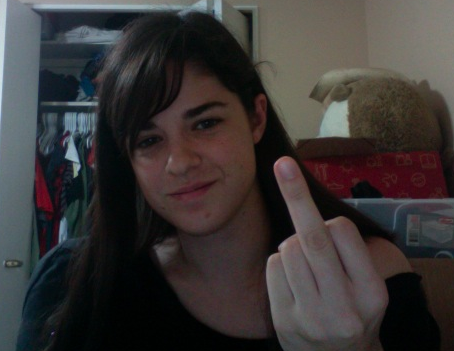
\includegraphics[width=5in]{./figures/made/Picture4.png}
%\end{center}

\cleardoublepage
%\newpage

% D E D I C A T I O N
% -------------------
%
%\begin{center}\textbf{Dedication}\end{center}
%
%This is dedicated to...
%\cleardoublepage
%\newpage

% T A B L E   O F   C O N T E N T S
% ---------------------------------
\tableofcontents
\cleardoublepage
%\newpage

% L I S T   O F   T A B L E S
% ---------------------------
%\listoftables
%\addcontentsline{toc}{chapter}{List of Tables}
%\cleardoublepage
%\newpage

% L I S T   O F   F I G U R E S
% -----------------------------
\listoffigures
\addcontentsline{toc}{chapter}{List of Figures}
\cleardoublepage
%\newpage

% L I S T   O F   S Y M B O L S
% -----------------------------
% \renewcommand{\nomname}{Nomenclature}
% \addcontentsline{toc}{chapter}{\textbf{Nomenclature}}
% \printglossary
%\cleardoublepage
% \newpage

% Change page numbering back to Arabic numerals
\pagenumbering{arabic}

 

%----------------------------------------------------------------------
% MAIN BODY
%----------------------------------------------------------------------
% Because this is a short document, and to reduce the number of files
% needed for this template, the chapters are not separate
% documents as suggested above, but you get the idea. If they were
% separate documents, they would each start with the \chapter command, i.e, 
% do not contain \documentclass or \begin{document} and \end{document} commands.
%======================================================================
% INTRODUCTION
%---------------------------
\chapter{Introduction}

%scaling\\
%universal quantities...\\
%The search for topological order\\
%looking at quantum critical points\\
%area law\\
%new attempts at entropies:\\
%- 
%\\

%According to G. Vidal: \\
%- the way tensor network states are constructed they can't have entropy scaling faster than area law\\

In this chapter we discuss different measures of entanglement and their scaling.
Then in Chapter 2 we describe quantum Monte Carlo algorithms in the valence bond basis.
Chapter 3 contains measurements of valence bond entanglement entropy as compared to standard von Neumann entanglement entropy.
In Chapter 4 we develop a method of measuring all Renyi entanglement entropies, excluding the von Neuman entanglement entropy, using valence bond quantum Monte Carlo.
In the final chapter we summarize the results of this research.

%---------------------------------------------------------------------------------------------------------
\section{Quantum Entanglement}
%---------------------------------------------------------------------------------------------------------
Entanglement is one important and interesting feature that differentiates quantum mechanical systems from classical systems.
In a pair of entangled spins/particles/photons/states the members of the system have information about each other, even if they are spatially separated.
Two spins, for instance, are considered entangled if their joint state can not be written as the product of their individual states.  Of the following two states,
\begin{equation}
	\ket{\Psi_{1,2}} = \frac{1}{\sqrt{2}} \big( \ket{\up_1\up_2} + \ket{\dw_1\dw_2}\big) 
	\hspace{1cm} \text{and} \hspace{1cm}
	\ket{\Phi_{1,2}} = \frac{1}{\sqrt{2}} \big( \ket{\up_1\dw_2} - \ket{\dw_1\dw_2}\big), 
\end{equation}
only $\ket{\Phi_{1,2}}$ is separable, and can be rewritten as
\begin{equation}
	\ket{\Phi_{1,2}} = \frac{1}{\sqrt{2}}  \big( \ket{\up_1} - \ket{\dw_1}\big) \otimes \ket{\dw_2}.
\end{equation}
In the case of only two spins it is easy to see that states are separable (unentangled). As we add more spins to the system it becomes less apparent which  states are entangled. Furthermore, we can quantify the degree to which they are entangled beyond being either separable states, or non-separable states (entangled).

%---------------------------------------------------------------------------------------------------------
\section{Measures of Entanglement}
%---------------------------------------------------------------------------------------------------------

There are many different quantities that can be used to measure entanglement. Though not exhaustive a few measures include concurrence, logarithmic negativity, squashed entanglement, and entropy of entanglement.
All measures of entanglement share three properties\cite{Plenio2005}:
\begin{enumerate}
\item A bipartite entanglement measure $E(\rho)$ (measuring the entanglement between two qubits) is a mapping from density matrices to positive real numbers defined for states of arbitrary bipartite systems.
Usually a normalization factor is included such that the maximally entangled state,
\begin{equation}
\ket{\psi_{\rm max}}  = \frac{\ket{0,0} + \ket{1,1}}{\sqrt{2}},
\end{equation}
 of two qubits has $E(\ket{\psi_{\rm max}}\bra{\psi_{\rm max}}) = \ln(2)$.
 \item  $E(\rho)=0$ if the state $\rho$ is separable.
 \item $E(\rho)$ does not increase under local operators on either of the qubits.  That is, if we have an operator acting on only {\it one} of the qubit, the entanglement between the two qubits will never increase.
% \item For a pure state $\ket{\psi}\bra{\psi}$ the measure reduces to the von Neumann entanglement entropy.
\end{enumerate}
There is also a fourth condition, not satisfied by all measures of entanglement, requiring the measure to reduce to the von Neumann entanglement entropy for a system in a pure state.


%---------------------------------------------------------------------------------------------------------
\section{The von Neumann Entanglement Entropy}
%---------------------------------------------------------------------------------------------------------
For a system partitioned into two regions, A and B, the von Neumann entanglement entropy \vn is defined as
\begin{equation}
	\VN_\text{A} = -\rm{Tr}\left({\rho_A \ln \rho_A}\right),
\end{equation}
where $\rho_{\rm{A}}=\rm{Tr}_B\ket{\psi}\bra{\psi}$ is the reduced density matrix, the density matrix of the entire system with the degrees of freedom from region B traced out.
\vn is only suited to measure the entanglement of a pure state, as is the case for all the entanglement measures we will discuss in this thesis.
This is due to the way \vn measures entanglement; we begin with a pure state and trace out the degrees of freedom for some subregion B.  
We are left with $\rho_{\rm A}$ representing a, possibly mixed, state.
\vn can be rewritten in terms of the eigenvalues of the density matrix,
\begin{equation}
\VN_\text{A} = -\sum_i \left(\lambda_i \ln \lambda_i\right),
\end{equation}
which is quite similar to the form of thermodynamic entropy or Shannon information entropy. If $\rho_{\rm A}$ represents a pure state we {\bf know} what state of region A is in, and $\rho_{\rm A}$ will have one non-zero eigenvalue equal to 1 (so $\VN = 0$).
If $\rho_{\rm A}$ represents a mixed state, we will have some probability distribution of the possible states (so $\VN > 0$). The entropy of that distribution is used to quantify the entanglement between regions A and B.
In the maximally entangled case all eigenvalues are equal to $1/d$ (representing an equal probability of encountering each spin state), where $d$ is the dimension of the Hilbert space for region A ($2^N$ for a system of $N$ spin-1/2 particles). Thus the maximum entanglement entropy for a spin-$1/2$ system is $\VN= \ln (d) = N \ln(2)$. 
If the initial state starts off mixed instead of pure, the state would already have some entropy. The entanglement entropy would contain both the initially present classical uncertainty in the state as well as that due to tracing out region B.

The von Neumann entanglement entropy is part of a larger class of entanglement entropies called the generalized Renyi entanglement entropies.
The $n^\text{th}$ Renyi entanglement entropy $S_n$ is defined as
\begin{equation} \label{renyi}
 	S_n(\rho_{\rm A}) = \frac{1}{1-n}\ln\left[{\rm Tr}\left( \rho_{\rm A}^n \right) \right].
\end{equation}
%It may not be immediately apparent that $\VN = S_1$, but if we take the limit as $n\to 1$,
%\begin{equation}
%S_1(\rho_{\rm A}) = \lim_{n\to1}\frac{\ln\left[{\rm Tr}\left( \rho_{\rm A}^n \right) \right]}{1-n}
%	=\lim_{n\to1}\frac{\frac{d}{dn}\ln\left[{\rm Tr}\left( \rho_{\rm A}^n \right) \right]}{\frac{d}{dn}(1-n)}
%\end{equation}
Taking the limit $n\to1$ gives us $S_1 = \VN$.  These entanglement entropies have the property that for $n>m$, $S_n\le S_m$; successive Renyi entropies give a lower bound on the previous entropies. They are useful measures to fully characterize the entanglement entropy of the system.

% \comment{cite some quantum information textbook}.


%---------------------------------------------------------------------------------------------------------
\section{Entanglement in Condensed Matter Systems}
%---------------------------------------------------------------------------------------------------------

Using measures of entanglement from quantum information to study interacting quantum many-body systems is a rapidly growing interdisciplinary topic \cite{Amico, intro}.
In systems that exhibit topological order, entanglement measures can be used to quantify ``hidden'' correlations \cite{wolf} and that order which is missed by standard measurements such as two-point correlation functions \cite{Bbob, KP, LW, Spectrum}.
Entanglement has the added benefit of being independent of the basis used to represent the condensed matter system.

%---------------------------------------------------------------------------------------------------------
\subsection{Scaling of Entanglement Entropy}
\label{1dcft}
%---------------------------------------------------------------------------------------------------------

The scaling of \vn is well understood in 1D systems \cite{ALreview} where, away from special critical points, entanglement between two regions scales as the size of the boundary between those regions.
This corresponds to systems with mainly short range entanglement, where only sites ``near'' the boundary contribute to the entanglement between regions.  
If we had a system with extremely long-range entanglement it would be expected that the entire region A is entangled with region B, and one would see a ``volume law'' scaling of entanglement. 
This ``area law'' \cite{Shredder} is expected to hold for the ground states of many interacting 2D quantum systems.



The scaling of entanglement entropy in 2D is also known to hold information about universal quantities.
In critical systems the area law scaling has universal additive logarithmic corrections \cite{Casini2007,Ryu}, and for topologically ordered systems there are universal additive constant corrections \cite{KP,LW}.

The 1D Heisenberg spin chain is critical, and the entanglement entropy is known to scale as \cite{Cardy} \cite{Zhou2006}
\begin{equation} \label{cft1d} 
	\VN_{\text{PBC}} = \frac{c}{3}\ln(x') + s_1
	\hspace{1cm}
	\VN_{\text{OBC}} = \frac{c}{6}\ln(2x') + \ln(g)+ \frac{s_1}{2}
\end{equation}
for systems with open and periodic boundary conditions, where $c$ is the central charge from conformal field theory, $g$ is a universal boundary term \cite{AffleckAndLudwig}, and $s_1$ is a model dependent constant. $x'$ is the conformal mapping for the number of sites included in region A, used to account for the finite size of the Heisenberg chains, when \eqref{cft1d} applies in the long chain-length limit.  $x \rightarrow x' = (L/\pi)\sin(\pi x/L)$ for PBC and $x \rightarrow 2x'$ for OBC, where L is the length of the chain.

For 2D Heisenberg spin systems with topological order, the entanglement entropy is known to scale as \cite{intro}
\begin{equation} \label{AL}
S_{\rm A} = \alpha \ell - n \gamma + \mathcal{O}(1/\ell),
\end{equation}
where $\ell$ is the length of the boundary, $\gamma$ is the topological entanglement entropy\cite{KP,LW}, and $n$ is related to the shape of the boundary.

\section{Measurement of Entanglement Entropy}

Many methods have been developed that are capable of measuring the entanglement entropy. In 1D DMRG and exact diagonalization are particularly powerful tools. They provide direct access to the density matrix and wavefunction. However exact diagonalization scales exponentially poorly as a function of system size and DMRG is primarily a tool useful for 1D and multi-leg ladders. To study and extract these universal quantities in 2D it is necessary to be able to measure entanglement entropy in a scalable type of simulation. New algorithms such as tensor-network states and projected entangled pair states, rely on states that are explicitly constructed to obey an area law \cite{MERA,PEPS1,PEPS2} but can scale to large system sizes. States scaling no faster than this area law can be accurately represented with matrix product states \cite{MPS_DMRG}. Quantum Monte Carlo is a method which scales well in any dimension and allows a choice of basis which is not constructed to obey any particular entanglement scaling relationships. In this thesis we explore methods of measuring entanglement entropy in quantum Monte Carlo simulations in the valence bond basis.



%======================================================================
%In the beginning there was $\pi$:
%\begin{equation}
%   e^{\pi i} + 1 = 0  \label{eqn_pi}
%\end{equation}
%----------------------------------------------------------------------
%\section{State of the Art}
%----------------------------------------------------------------------
%See equation \ref{eqn_pi} on page \pageref{eqn_pi}.\footnote{A famous equation.}


%======================================================================
\chapter{Quantum Monte Carlo in the Valence Bond Basis}
%======================================================================

\section{Single Projector}
\section{Double Projector}
\section{Loop Moves}

%This would be a good place for some figures and tables.

%Some notes on figures and photographs\ldots

%\begin{itemize}
%\item A well-prepared PDF should be 
%  \begin{enumerate}
%    \item Of reasonable size, {\it i.e.} photos cropped and compressed.
%    \item Scalable, to allow enlargment of text and drawings. 
%  \end{enumerate} 
%\item Photos must be bit maps, and so are not scaleable by definition. TIFF and
%BMP are uncompressed formats, while JPEG is compressed. Most photos can be
%compressed without losing their illustrative value.
%\item Drawings that you make should be scalable vector graphics, \emph{not} 
%bit maps. Some scalable vector file formats are: EPS, SVG, PNG, WMF. These can
%all be converted into PNG or PDF, that pdflatex recognizes. Your drawing 
%package probably can export to one of these formats directly. Otherwise, a 
%common procedure is to print-to-file through a Postscript printer driver to 
%create a PS file, then convert that to EPS (encapsulated PS, which has a 
%bounding box to describe its exact size rather than a whole page). 
%Programs such as GSView (a Ghostscript GUI) can create both EPS and PDF from PS files.
%Appendix~\ref{AppendixA} shows how to generate properly sized Matlab plots and save them as PDF.
%\item It's important to crop your photos and draw your figures to the size that
%you want to appear in your thesis. Scaling photos with the 
%includegraphics command will cause loss of resolution. And scaling down 
%drawings may cause any text annotations to become too small.
%\end{itemize}
% 
%For more information on \LaTeX\, see the UW Skills for the Academic Workplace 
%course notes at \href{http://saw.uwaterloo.ca/latex}{saw.uwaterloo.ca/latex}. 
%\footnote{
%Note that while it is possible to include hyperlinks to external documents,
%it is not wise to do so, since anything you can't control may change over time. 
%It \emph{would} be appropriate and necessary to provide external links to 
%additional resources for a multimedia ``enhanced'' thesis. 
%But also note that if the \package{hyperref} package is not included, 
%as for the print-optimized option in this thesis template, any \cmmd{href} 
%commands in your logical document are no longer defined.
%A work-around employed by this thesis template is to define a dummy \cmmd{href} 
%command (which does nothing) in the preamble of the document, 
%before the \package{hyperref} package is included. 
%The dummy definition is then redifined by the
%\package{hyperref} package when it is included.
%}

%The classic book by Leslie Lamport \cite{lamport.book}, author of \LaTeX , is worth a look too, 
%and the many available add-on packages are described by 
%Goossens \textit{et al} \cite{goossens.book}. Some on-line documentation is linked
%to from \href{http://saw.uwaterloo.ca/latex}{saw.uwaterloo.ca/latex}.

%======================================================================
\chapter{Valence Bond Entanglement Entropy}
%======================================================================
\section{One Dimension}
\section{Approaching Two Dimensions}
\section{The Area Law}

%======================================================================
\chapter{Measuring R\'{e}nyi Entanglement Entropy}
%======================================================================
\section{The Swap Operator}
\section{1D Results}
\section{The Ratio Operator}
\section{2D Results}
\section{The Area Law}


%======================================================================
\chapter{Prospects for Future Research}
%======================================================================
%======================================================================
\chapter{Conclusions}
%======================================================================

% The \appendix statement indicates the beginning of the appendices.
\appendix
% Add a title page before the appendices and a line in the Table of Contents
\chapter*{APPENDICES}
\addcontentsline{toc}{chapter}{APPENDICES}
%======================================================================
%\chapter[PDF Plots From Matlab]{Matlab Code for Making a PDF Plot}
%\label{AppendixA}
% Tip 4: Example of how to get a shorter chapter title for the Table of Contents 
%======================================================================
%\section{Using the GUI}
%Properties of Matab plots can be adjusted from the plot window via a graphical interface. Under the Desktop menu in the Figure window, select the Property Editor. You may also want to check the Plot Browser and Figure Palette for more tools. To adjust properties of the axes, look under the Edit menu and select Axes Properties.

%To set the figure size and to save as PDF or other file formats, click the Export Setup button in the figure Property Editor.

%\section{From the Command Line} 
%All figure properties can also be manipulated from the command line. Here's an example: 
%\begin{verbatim}
%x=[0:0.1:pi];
%hold on % Plot multiple traces on one figure
%plot(x,sin(x))
%plot(x,cos(x),'--r')
%plot(x,tan(x),'.-g')
%title('Some Trig Functions Over 0 to \pi') % Note LaTeX markup!
%legend('{\it sin}(x)','{\it cos}(x)','{\it tan}(x)')
%hold off
%set(gca,'Ylim',[-3 3]) % Adjust Y limits of "current axes"
%set(gcf,'Units','inches') % Set figure size units of "current figure"
%set(gcf,'Position',[0,0,6,4]) % Set figure width (6 in.) and height (4 in.)
%cd n:\thesis\plots % Select where to save
%print -dpdf plot.pdf % Save as PDF
%\end{verbatim}

%----------------------------------------------------------------------
% END MATERIAL
%----------------------------------------------------------------------

% B I B L I O G R A P H Y
% -----------------------

% The following statement selects the style to use for references.  It controls the sort order of the entries in the bibliography and also the formatting for the in-text labels.
\bibliographystyle{plain}
% This specifies the location of the file containing the bibliographic information.  
% It assumes you're using BibTeX (if not, why not?).
\bibliography{thesis}
% The following statement causes the title "References" to be used for the biliography section:
\renewcommand{\bibname}{References}
\addcontentsline{toc}{chapter}{\textbf{References}}
% Tip 5: You can create multiple .bib files to organize your references. 
% Just list them all in the \bibliogaphy command, separated by commas (no spaces).

% The following statement causes the specified references to be added to the bibliography% even if they were not 
% cited in the text. The asterisk is a wildcard that causes all entries in the bibliographic database to be included (optional).
\nocite{*}

\end{document}
